\documentclass[tikz,border=5pt]{standalone}
\usepackage{amsmath}
\usepackage{tikz}
\usetikzlibrary{arrows.meta}
\definecolor{nebula}{HTML}{6366F1}
\definecolor{spark}{HTML}{14B8A6}
\definecolor{ink}{HTML}{334155}
\begin{document}
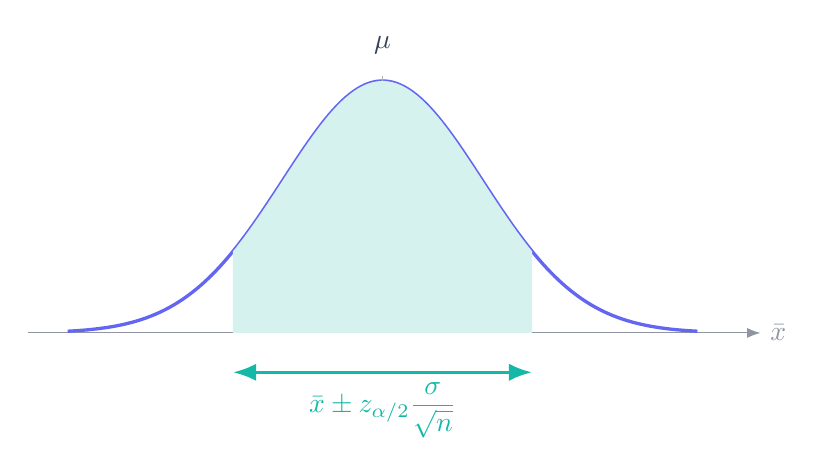
\begin{tikzpicture}[font=\sffamily,>=Latex,x=1cm,y=1cm]
  \draw[->,ink!55] (-4.5,0)--(4.8,0) node[right] {$\bar x$};
  \draw[domain=-4:4,samples=160,very thick,nebula] plot(\x,{3.2*exp(-\x*\x/3.2)});
  \draw[dashed,ink!40] (0,0)--(0,3.3);
  \fill[spark!18] (-1.9,0)--plot[domain=-1.9:1.9,samples=80](\x,{3.2*exp(-\x*\x/3.2)})--(1.9,0)--cycle;
  \draw[<->,very thick,spark] (-1.9,-.5)--(1.9,-.5);
  \node[spark,below] at (0,-.5) {$\bar x\pm z_{\alpha/2}\dfrac{\sigma}{\sqrt n}$};
  \node[ink] at (0,3.65) {$\mu$};
\end{tikzpicture}
\end{document}
